\documentclass[12pt]{article}
\usepackage{scicite}
\usepackage{times}
\usepackage{graphicx}
\usepackage{color}
%\usepackage{changes}
\usepackage[final]{changes}


\topmargin 0.0cm
\oddsidemargin 0.2cm
\textwidth 16cm 
\textheight 21cm
\footskip 1.0cm

\newenvironment{sciabstract}{%
\begin{quote} \bf}
{\end{quote}}

\renewcommand\refname{References and Notes}

\newcounter{lastnote}
\newenvironment{scilastnote}{%
\setcounter{lastnote}{\value{enumiv}}%
\addtocounter{lastnote}{+1}%
\begin{list}%
{\arabic{lastnote}.}
{\setlength{\leftmargin}{.22in}}
{\setlength{\labelsep}{.5em}}}
{\end{list}}


\title{Cross-contaminated cell lines weaken the US Patent Database} 

\author
{Iva Bojic,$^{1,2\ast}$ Jessica Snyder,$^{1}$ Aaron Gerow$^{2}$, Richard M. Neve$^{4}$, Carlo Ratti$^{1}$ \\
\\
\normalsize{$^{1}$Massachusetts Institute of Technology, SENSEable City Lab, Cambridge, Massachusetts 02139, USA}\\
\normalsize{$^{2}$Singapore-MIT Alliance for Research and Technology, SENSEable City Lab, Singapore}\\
\normalsize{$^{3}$The University of Chicago, Knowledge Lab, Chicago, Illinois 60637, USA}\\
\normalsize{$^{4}$Gilead Sciences, Foster City, California 94404, USA}\\
\\
\normalsize{$^\ast$To whom correspondence should be addressed; E-mail ivabojic@mit.edu.}
}

\begin{document} 

\baselineskip24pt
\maketitle 

\begin{sciabstract}
Including false data in a United States Patent, with or without the knowledge of the inventor, infringes the inventor's oath of truthfulness and may enable the patent to be later challenged. Inventors continue to cite contaminated or misidentified cell lines in patent application, despite contamination problems dating back to the first established cell lines in the early 1950's. Recent efforts to eradicate the use of misidentified and cross-contaminated cell lines in published research appear to be working as the percentage of research using ``false'' cell lines shows the tendency to drop. At the same time, possibly due to a lack of the control, \replaced{citations}{ the usage} of ``false'' cell lines in \replaced{US approved patents}{ filled patents } has increased. The continued acceptance of patents citing false cells lines makes the system vulnerable to lengthly, costly legal battles if the citation is found and challenged by a competitor. 
\end{sciabstract}

 \newpage

\section*{US patent database weakened by false cell lines}
Including false data in a United States Patent, with or without the knowledge of the inventor, infringes the inventor's oath of truthfulness and may enable the patent to be later challenged.

\textit{"In the United States, in contrast to many other countries, inventors must sign a declaration affirming that everything in their application is true to the best of their knowledge. The inclusion of false data, even by mistake, could be an infringement of the oath, and thus against the law. Or it could form the basis for questioning the patent later, says Alan Grimaldi, co-chair of the intellectual-property group at Howrey law firm in Washington DC."  \textbf{From Reich, E.S. Bad data fail to halt patents. Nature. 439, 379 (26 January 2006) }}

Mistaken identify compromises one of the most commonly used laboratory model system for drug manufacturers and basic medical research.

\section*{A 50+ year old issue}

In 1952, after decades of attempts, George Gey successfully harvested robust, immortal cells that enabled him to establish the first human cancer cell line \cite{gey1952tissue}. Gey was generous in sharing his findings and sending extracted cells all around the world \cite{culliton1974hela}. However, exactly the same characteristics that helped Gey bring HeLa to life, were responsible for the cells rapidly overgrowing other cells, resulting in contamination in labs across the world \cite{chatterjee2007cases}. At first, it was difficult to distinguish between cell lines derived from different individuals of the same species, but by the early 1980s, Nelson-Rees relentlessly pursued and exposed intrahuman (HeLa and non-HeLa) and interspecies cross-contamination, publishing a comprehensive list of nearly 100 cross-contaminated cell lines \cite{nelson1976hela, nelson1981cross}.

In the years that followed, many studies showed similar results, but received less attention until major world cell banks decided to act by informing clients or even withdrawing ``false'' cell lines from their catalogs. The Deutsche Sammlung von Mikroorganismen und Zellkulturen pioneered the process in 1999 where they tested 252 human tumor cell lines stored in their repository and found that 18\% of cell lines were cross-contaminated \cite{macleod1999widespread}. This was followed by examining 550 human leukemia-lymphoma cell lines in 2003 where unequivocal evidence showed misidentification for 15\% of them \cite{drexler2003false}. Around the world, other repositories such as Cell Engineering Division of the Japanese research institution RIKEN \cite{yoshino2006essential} and National Cell Bank of Iran \cite{azari2007profiling} followed suit finding similar results.

\section*{Measuring the problem's modern scope}
We searched through manuscripts available from PubMed and SCOPUS databases as well as through the US patent database for instances of 3,508 cell lines identified in previous research \cite{yu2015resource} (See Supplementary Materials). During the last 15 years, the percentage of published manuscripts in which ``false'' cell lines were used shows the tendency to fall. For the same period, the percentage of filed patents citing misidentified and cross-contaminated cell lines has risen (Figure \ref{fig1}).

The most comprehensive database of misidentified and cross-contaminated cell lines lists 488 lines in which 451 cell lines were misidentified ``early''. For these, no known authentic stock exists. The remaining 37 cell lines were misidentified ``late'', where a tested sample had been overgrown, but authentic stock was found \cite{capes2010check}. Originally published in 2010, the database is now curated by the International Cell Line Authentication Committee. A recent AAAS/Science Magazine and Sigma-Aldrich's survey\footnote{http//go.sigmaaldrich.com/Translational-Survey} found that less than half of survey respondents \replaced{were}{ was } familiar with the database, and only 11\% had used it during the preceding year. This would not be a problem if other studies did not show that between 63\% \cite{buehring2004cell} and 69\% \cite{shannon2016cell} survey respondents obtained at least one cell line from their colleagues (i.e. other research laboratories). When cell lines are obtained from colleagues, they typically lack verification or documentation about the condition or past number of the lines. There is thus an increasing chance that contamination goes unnoticed. Results from three independent studies are conclusive that nearly half of respondents never tested the identity of lines they used \cite{buehring2004cell, shannon2016cell, freedman2014culture}.

But is the number of available misidentified and cross-contaminated cell lines a good proxy for what scientists actually use in research? Until now, certain studies reported only on the misuse of a small subset of mostly HeLa-contaminated cell lines in scientific literature. In 2004 the authors searched through scientific literature on PubMed extending from 1969 to 2004 to find that in 220 published manuscripts one or more of 13 HeLa-contaminant cell lines were used as models for the tissue type of the original cell line \cite{buehring2004cell}. One year later, it was reported that 1,149 manuscripts published between 2000 and 2004 used one of six contaminated HeLa lines, a problem to which fewer than 10\% admitted \cite{masters2005dna}.

\added{Let's acknowledge a misindentified or cross-contaminated cell line is scientifically credible as a general model of cell behavior or to produce virus, but not valid to represent the specific tissue of the cell line's original biopsy.} \deleted{The important thing here to note is that not every occurrence of a cell line, which is listed in} \added{Therefore, publications which mention cell lines from the misidentified and cross-contaminated database cannot be outright dismissed as bad science.} \deleted{misidentified and cross-contaminated database in a manuscript or a patent necessary immediately do not means its misuse} \deleted{Namely, although a certain cell line is listed in the aforementioned database, it can be used for a general purpose to produce for example study cell biology or chemistry.} In order to get the full picture, one would need to ascertain whether the use of the cell line was tissue specific or not. The results of previous studies, although limited by the number of cell lines they took into a consideration, gave insights that in a small portion of manuscripts authors acknowledged they were aware of contamination (e.g. fewer than 10\% \cite{masters2005dna}). Due to the \replaced{large}{ extent of the } number of manuscripts and patents in our database, it was impossible to go manually through \replaced{each one}{ every of them } as it was done in the previous studies. However, following the methodology described in Supplementary Materials, we \replaced{estimated less than}{ concluded that only} 10\% of patents and 18\% of manuscripts \deleted{ possibly} acknowledged that \replaced{they knowingly used}{ they were aware of using } misidentified or cross-contaminated cell lines in their research. \added{Many publications fail to use properly identified cell lines known to be free of contamination, and when authors do use contaminated cell lines, most fail to cite the findings cannot be used to characterize a specific tissue.} 

\section*{More accepted patents cite false cell lines each year}


\begin{figure*}[b!]
\centering
	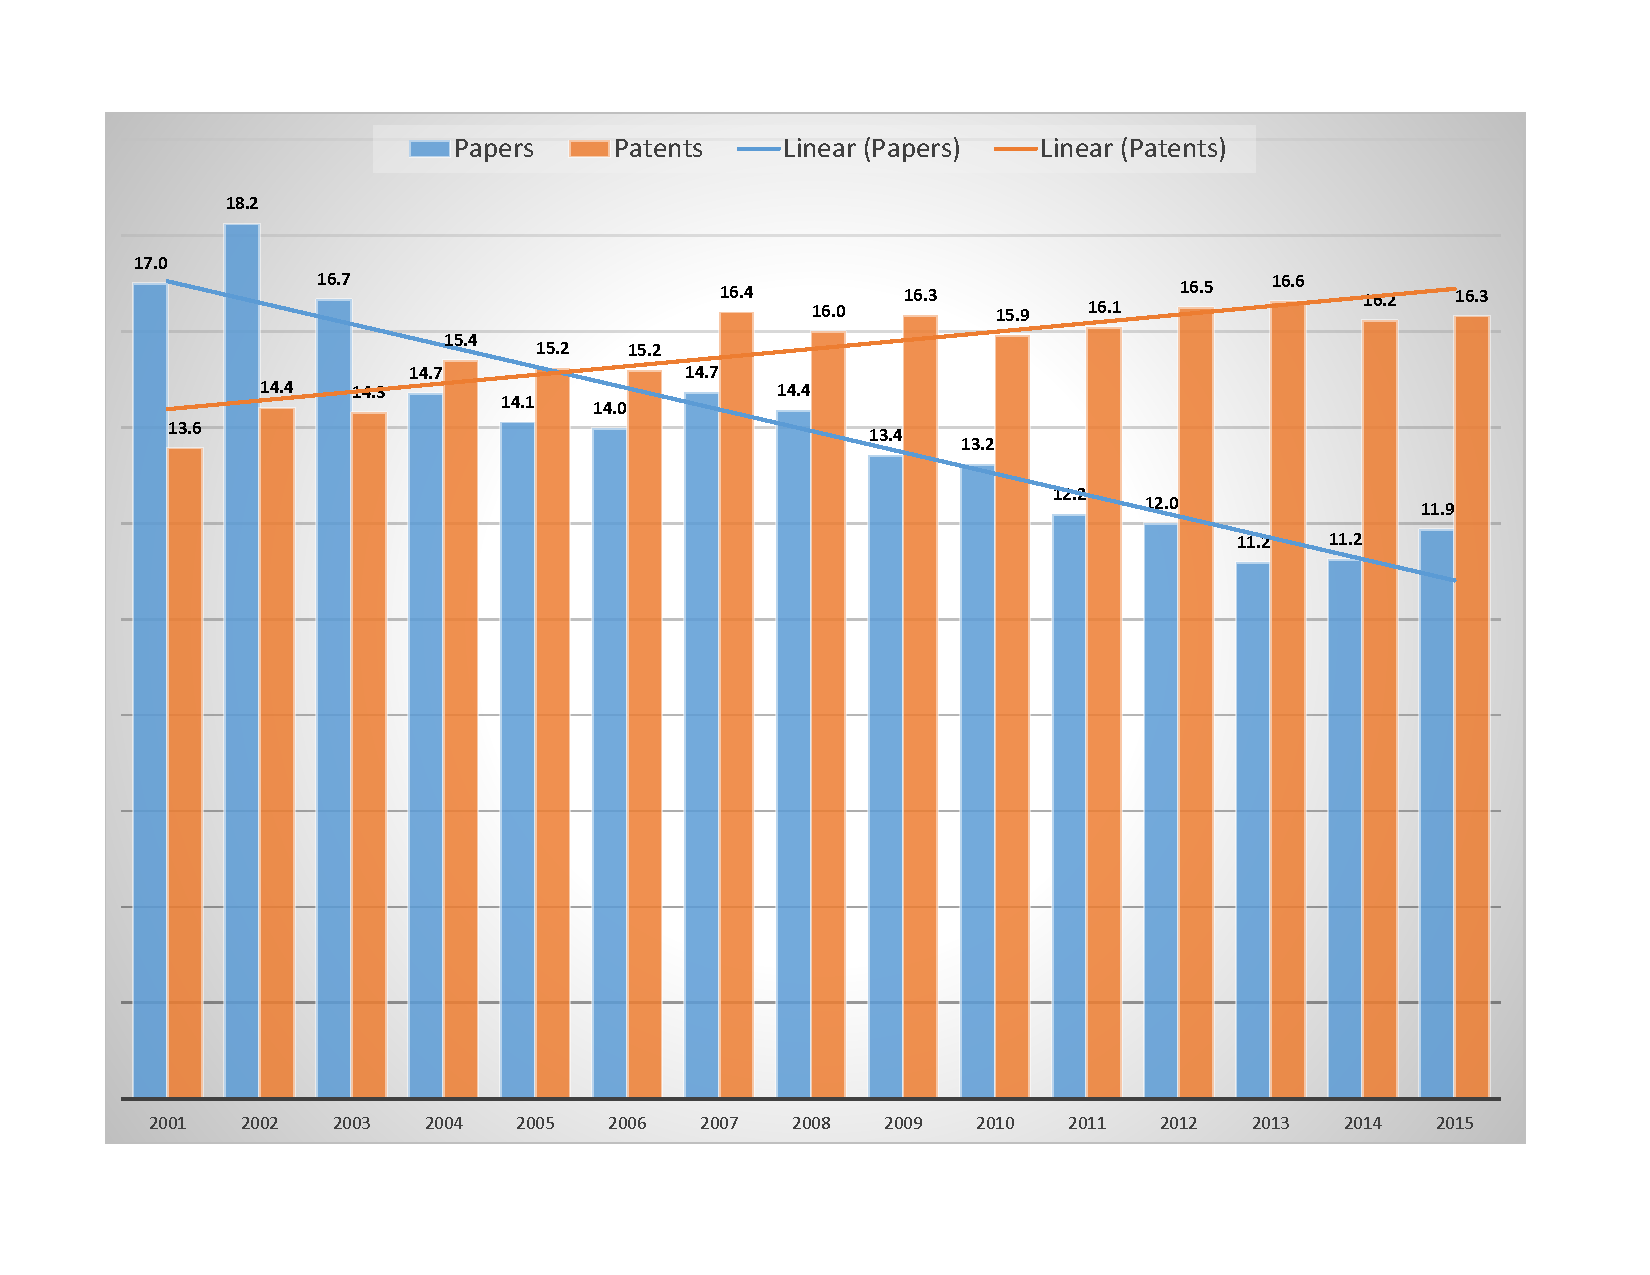
\includegraphics[width=.75\textwidth]{Graph.pdf}
	\caption{\label{fig1}Percentage of manuscripts published and patents filed between 2001 and 2015 citing misidentified or cross-contaminated cell lines.}
\end{figure*}


\section*{Direct action reduced citations in publications}

Since \added{many} scientific \replaced{publishers}{ community } \replaced{have}{ was } not \replaced{authenticated the cell line's efficacy}{able to tackle cell line contamination} for over 50 years \deleted{now}, it is not surprisingly that this problem has been described as the most compelling quality-control issue confronting the community \cite{nardone2008curbing}. The ``false'' cell lines have already been unwittingly used in several hundreds of potentially misleading reports, including use as inappropriate tumor models and subclones masquerading as independent replicates. However, this study provides us with comforting results that over time researchers have been able to reduce the percentage of misidentified and cross-contaminated cell lines cited in manuscripts. 

Looking retrospectively, \replaced{elevating scientific rigor took}{ all it took was for } a group of brave scientists to raise their voices. Gartler was the first, when in 1967, he reported 18 human cell lines supposedly of independent origins were all, in fact, HeLa cells \cite{gartler1967genetic}. However, his findings were not well received by in the scientific community, but one researcher went into open battle to expose the problem: Nelson-Rees. In the 1970s, as Nelson-Rees ran a cell bank at Berkeley under contract for the National Cancer Institute, he was ideally positioned to expand Gartler's findings in a series of publications in \textit{Science}\cite{nelson1976hela, nelson1981cross, nelson1974banded}. Publishing in on this topic certainly did not help his career because in the same year, a \textit{Nature} referred to him as a ``\textit{self-appointed vigilante}'' \cite{maddox1981responsibility} after which his contract was terminated by the NIH and he gave up science to open an art gallery in San Francisco. 

The third crusade began in 2004 lead by Nardone\added{,} who had been educating at the NIH about cell culture techniques for more than two decades \cite{nardone2007eradication}. His white paper advocated two broad changes: more regulation and increased education efforts from different professional societies. The regulation effort should come both from funding agencies, which should require cell lines authentication to receive funds, and journals, which should not publish manuscripts using cell lines not previously authenticated. Similarly, publication of new cell lines by originators, or the funding of their production should be conditional on the lines being authenticated and made freely available to other investigators (e.g. in cell banks). Over time, it was realized that resolution of the problem of misidentification and cross-contamination requires the collaboration of other stakeholders in addition to funding agencies and publishers---it should involve users (including originators) of cell lines, cell banks / distributors, reviewers for journals and funding agencies, laboratory directors, etc.. 

In the late 2000s, journals like \textit{Cell Biochemistry and Biophysics}, \textit{In Vitro Cellular \& Developmental Biology} and \textit{International Journal of Cancer} began requiring all cell lines be authenticated before publication \cite{american2010cell}. From 1 May 2015, all authors of manuscripts involving cell lines that are submitted to Nature journals have been asked whether they authenticated their cell lines \cite{editorial2015time}. To date, more than 70 journals have guidelines for cell line authentication prior to publication\footnote{http//www.celllineauthentication.com/journal-requirements.html}. Almost simultaneously with journals changing their policies, cell banks have begun to change their attitude as well. However, \replaced{reform took}{ it had to past } almost ten years\added{,} from Stacey's recommendation on a clear identification of cross-contaminated cultures in catalogue entries of culture collections \cite{stacey2000cell}\added{,} \replaced{to when }{ for it to become a reality in 2010 when} the database of misidentified and cross-contaminated cell lines was created \added{in 2010,} \cite{capes2010check} followed by ATCC, CellBank Australia, sDSMZ, ECACC, JCRB, and RIKEN publishing the same list on their websites.

\section*{Zero tolerance for false cell lines from NIH}
The slowest adopter in the process was NIH, whose role was twofold: providing proper education and adopting zero tolerance policy on funding research that uses misidentified and cross-contaminated cell lines \cite{lorsch2014fixing}. With its efforts to enhance reproducibility, NIH developed a training module emphasizing good experimental design, which is now incorporated into the mandatory training on responsible conduct of research for NIH intramural postdoctoral fellows \cite{collins2014nih}. This is very much needed, as the recent study showed that when it comes to training, only 62\% of survey respondents had received specific training on the problems of cell line misidentification and cross-contamination, while less than 30\% were trained the importance of cell line authentication as a quality control measure for species confirmation \cite{freedman2014culture}. Finally, beginning in 2016, ``\textit{NIH expects that key biological and / or chemical resources are regularly authenticated to ensure their identity and validity for use in the proposed studies}''\footnote{http//grants.nih.gov/grants/guide/notice-files/NOT-OD-15-103.html} \replaced{This is a step toward a well-defined mandate for}{, whereas the current gold standard for human cell line authentication is Short Tandem Repeats (STR)} genotyping \added{by the current authentication standard, Short Tandem Repeats (STR)}\cite{masters2012authentication}.

However, it is alarming that in the whole body of research on misidentified and cross-contaminated cell lines, only a few scholars showed concern for the usage of ``false'' cell lines in patents. Namely, the only occurrence found was in the manuscript from 1998 in which Markovic \& Markovic said ``\textit{filing patents and product licensing may also be compromised}'' \cite{markovic1998cell}. In this paper we have indeed showed that more than 15\% of patents filled in 2015 cited one of misidentified and cross-contaminated cell lines, which is 5\% more than for manuscripts.

\section*{Conclusions}
To this end, it is important to bare in mind the impact of cell culture contamination extends far beyond the relatively narrow field of cytobiology and the researchers studying cell lines and can for example also \replaced{falsely steer}{ affect} radiobiologists investigating certain topics in their field \cite{lucey2009henrietta}. The fight with misidentified and cross-contaminated cell lines so far, has certainty inspired changes in stakeholeders' attitudes and with the recent adoption of new ANSI / ATCC standards and NIH best practices, researchers will be able to allocate dedicated funds for the authenticity check. Namely, it has already been estimated that purchasing cell lines from a reputable vendor and authenticating them annually would cost only about 0.2\% of the budget for an NIH funded project \cite{freedman2015economics}. 

With the increasing number of scientific journals, editors requiring or recommending cell line authentication as condition for publication and availability of education materials on this matter, in the last 15 years we were able to reduce the percentage of published manuscripts using ``false'' cell lines to almost 10\%. This still implies that more than \$350 million dollars are wasted on research annually as estimated in \cite{freedman2014culture, freedman2015economics}. However, what is most worrying is not that more than 15\% of cell lines used in patents are ``false'', but also that this percentage is growing. This trend could possible indicate that we would need to have a better control over cell lines used in research filled for patents.

\section{Supplementary Materials \& Methods}
A set of 644,018 manuscripts published from 1970 to 2016 was selected from medline\footnote{\textit{www.ncbi.nlm.nih.gov/pubmed}; leased data, bulk download.} and PubMed Central\footnote{\textit{www.ncbi.nlm.nih.gov/pmc}; by API.} by one of the six following Medical Subject Headings (MeSH) terms\footnote{\textit{www.ncbi.nlm.nih.gov/mesh}} \textit{Cell Line}, \textit{Cell Line, Transformed}, \textit{Cell Line, Tumor}, \textit{Breast Neoplasms}, \textit{Prostatic Neoplasms} and \textit{Lung Neoplasms}. The first three MeSH terms were chosen because they contained the term \textit{cell line} and last three because breast, prostate and lung have been the top three cancer sites since the early 1990's\footnote{\textit{www.cancer.org/research/cancer-facts-statistics/all-cancer-facts-figures/cancer-facts-figures-2017.html}}. From this set, 169,464 full text versions were available from PubMed Central or SCOPUS\footnote{\textit{www.scopus.com}; proprietary API access.}. A second dataset of consisted of 4,568,258 patents selected from the entirety of the US Patents\footnote{\textit{www.uspto.gov}; weekly bulk downloads.} from January 2001 to May, 2016 by searching for forms of the word \textit{cell} in the text and supporting documentation.

A set of 3,508 cell lines of human origin (i.e. \textit{homo sapiens}) with unique names was compiled using data from Supplementary Table 2 and Supplementary Table 6 included in \cite{yu2015resource}. Namely, of 3,515 human cell lines, seven were listed twice: 2B8, AC-1M46, FTC-236, HKB-11, I 9.2, NCI-N417, P3HR-1. We mapped twelve potential Contaminant Statuses to either 1, denoting contaminated cell lines, or 0 denoting non-contaminated (Supplementary Table 3). \textit{Parental}, \textit{Parental?}, \textit{Derivative Line} and \textit{Derivative Line?} statuses were only considered for cell lines whose \textit{Name} and \textit{Canonical Name} were different, otherwise we mapped them to 0 (see Supplementary Table 2). The entire list of cell lines is shown in Supplementary Table 1.

Once when we had the whole list in Supplementary Table 1, we extracted cell line Names (i.e. the first column) from the downloaded manuscripts and patents. Variation in cell line nomenclature was accommodated by allowing a space, '-', '/' or parentheses between transitions of alphabetic and numeric characters (and vice versa) and where a delimiting character occurred in the canonical name. This collapses, for example, \textit{MCF(7)}, \textit{MCF7}, \textit{MCF 7} and \textit{MCF-7}, into the canonical form \textit{MCF-7}. This matching procedure found 136,855 manuscripts that mentioned one or more cell lines, with a total of 2,767,589 instances overall. 181,283 patents mentioned one or more cell lines and a total of 2,829,331 cell line occurrences was found. After collapsing all instances of the same cell line in a certain manuscript / patent, 552,006 and 850,116 unique cell line occurrences remained in manuscripts and patents, respectively. 

To exclude false positives, we examined the frequency distribution of cell lines occurring in a manuscripts and patents. Approximately 50\% of our records are of a cell line found only once in a particular manuscript / patent ( Supplementary Table 4). There is a good chance these mentions are false positives, which motivated removing mentions of cell lines with fewer than two mentions. This means we only consider instances that repeated two or more times in the same manuscript or patent. After applying this criteria, 52\% and 45\% of unique cell lines occurrences in manuscripts and patents remained, respectively. Because the chance a record is a false positive is correlated with the length of cell line name (44 cell line names have only two characters), we used a threshold of three. The final dataset included 233,656 unique manuscripts and 315,502 patents.

From the set of 259 parental cell lines, we chose 26 of cell lines whose parental line was HeLa (Supplementary Table 5) to assess the percentage of research acknowledging the contamination problem. We chose HeLa as a parental cell line because according the database of cross-contaminated or misidentified cell lines \cite{capes2010check} HeLa is the most common. Here, it is important to note that if research requirement was for any human cell line, then it is not important whether it was HeLa or another cell line. However, in those cases where it was assumed that a specific tissue origin of the cell line was used and cell line was in fact cross-contaminated or misidentified, the work is dubious. We found 3,423 unique manuscripts and 4,579 patents cite one of 26 cell lines from Supplementary Table 5. However, only 610 manuscripts and 478 patents also mentioned HeLa. Although, the authors could acknowledge they were aware of contamination without explicitly mention HeLa, this is likely a small portion of research.

\bibliography{scibib}

\bibliographystyle{Science}

\end{document}
